\documentclass[11pt, spanish]{article}
\usepackage[spanish, activeacute]{babel}
\usepackage[utf8]{inputenc}
\usepackage{graphicx}
\usepackage{algorithm}
\usepackage{algorithmic}
\usepackage{fullpage}
\renewcommand{\baselinestretch}{1.3}
\floatname{algorithm}{Algoritmo}

\begin{document}
\title{Introducción a la Programación Multinúcleo\\Evolución genética de imágenes}
\author{
  Daniel Barreto - \#04-36723 \texttt{<daniel@gia.usb.ve>}\\
  Ernesto Level - \#05-38402 \texttt{<ealevel@gmail.com>}
}
\date{\today}

\maketitle

\begin{figure}[htp]
  \centering
  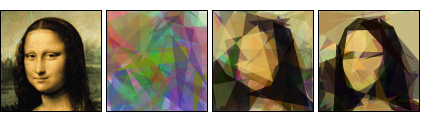
\includegraphics[scale=0.7]{media/evolution.png}
\end{figure}

\section{Introducción}
El presente trabajo expone la utilización de un algorítmo genetico
para ``evolucionar'' la mejor aproximación hacia una imagen usando una
cantidad finita de polígonos sobrepuestos y semi-transparentes, y
estudiar el comportamiento del algorítmo en la arquitectura
\textbf{Cell Broadband Engine} de IBM.

\subsection{Evolucionando imágenes}
La ``evolución de una imagen'', en el contexto de este proyecto,
consiste en conseguir configuraciones de un número estático y finito
de polígonos (dado como un parámetro del algorítmo) para aproximarse a
una represetación de una imágen dada a través de técnicas de
programación evolutiva.\\

Una configuración de poligonos está dada como una lista de polígonos
semi-transparentes sobrepuestos entre ellos, siendo dibujados en el
orden en el que salen en la lista.\\

Por su parte, los polígonos estan representados simplemente como una
secuencia de vertices, un color de base (en formato \textbf{RGB}) y un
nivel de transparencia \texttt{alpha}.\\

De esta forma, la estrategia evolutiva del algorítmo es usar las
nombradas configuraciones como individuos a evolucionar, tratando de
mejorar su función de \emph{fitness}, la cual es explicada más
adelante en la sección \ref{subsec:fitness}

\section{Marco teórico}
\subsection{Algorítmos genéticos}
Los algorítmos genéticos son parte de una línea de estudio en la
\emph{inteligencia artificial}, son llamados asi porque ``se inspiran en
la evolución biológica y su base genético-molecular. Estos algoritmos
hacen evolucionar una población de individuos sometiéndola a acciones
aleatorias semejantes a las que actúan en la evolución biológica
(mutaciones y recombinaciones genéticas), así como también a una
Selección de acuerdo con algún criterio, en función del cual se decide
cuáles son los individuos más adaptados, que sobreviven, y cuáles los
menos aptos, que son descartados.''\cite{wiki}.\\

Una representación generalizada de un algoritmo genético se encuentra más
detallada en el algoritmo \ref{genetic}.

\subsection{Investigaciones previsa y aproximaciones al problema}
Hasta el momento se han realizado dos estudios para buscar la solución
de la evolución de imagenes. Estas han sido realizadas por Roger
Alsing\cite{roger}, pionero en la idea de conseguir aproximaciones a
una imagen usando polígonos, y Jacob Seidelin\cite{jacob}.

\begin{enumerate}
\item \textbf{Roger Alsing:} Utiliza una población de sólo un
  individuo, que representa una cantidad de polígonos variable,
  empieza con un único polígono y luego va agregando mas. Realiza
  mutaciones con poca probabilidad para ir variando las posiciones y
  los colores de los polígonos que representa el individuo. Parecido a
  \emph{Hill Climbing}

\item \textbf{Jacob Seidelin:} Utiliza una población variable, pero de
  más de un individuo. Los individuos con mejor fitness se cruzan y se
  generan nuevas poblaciones. Aproximación netamente genética.
\end{enumerate}

\subsection{Estructuras y representaciones genotipos}
Para la implementación realizada, la cual es explicada en la sección
\ref{sec:implementacion}, se utilizó una lista de números
\emph{flotantes} entre $[0, 1]$ (ambos inclusive) para representar el
\emph{ADN} de un individuo. Esta lista de flotante contiene, o
representa, a su vez una secuencia de polígonos, que son los elementos
claves de cada \emph{ADN}.\\

Un polígono está dado como: un color (r, g, b), un nivel de transparencia u
opacidad y una secuencia de puntos (x, y) que representan sus
vertices. Luego la lista de flotantes que representa a un polígono es
de la siguiente forma:

\begin{verbatim}
r g b a v1x v1y v2x v2y ... vNx vNy
\end{verbatim}

Dónde cada item es un número flotante. Luego podemos calcular que el
tamaño de la representación de un polígono es: $4 + 2 * numero\ de\
vertices$, y de la misma forma, podemos ver que el tamaño de la lista
de flotantes de un \emph{ADN} es: $(4 + 2 * numero\ de\ vertices) *
numero\ de\ poligonos$

\section{Implementación}
\label{sec:implementacion}
Como ya se ha dicho anteriormente, para la resolución de este problema
se utilizó un algoritmo genético, éste parte de la creación de una
población de individuos generados aleatoriamente.\\

A partir de esta población se genera una nueva, esto se hace tomando
los mejores individuos para realizar en ellos los \emph{operadores
  genéticos} de recombinación y mutación. Esta nueva población
generada toma el lugar de la población anterior, y en caso que el
mejor individuo de esa población sea el mejor individuo encontrado
hasta el momento, se dibuja. Este último de paso se hace un número no
determinado de veces, dependiendo de que tan bien estén saliendo los
individuos de las nuevas generaciones. Mientras más veces se realice,
mejores individuos se van consiguiendo y mejor la solución generada se
parece más a la imagen original.\\

\subsection{Variables aleatorias del algoritmo}
El algoritmo implementado contiene \textbf{6} variables aleatorias, las
cuales son explicadas a continuación:

\begin{enumerate}
\item \textbf{Tamaño de la imagen:} El tamaño en pixeles de la imagen,
  para este proyecto se usan solo imágenes cuadradas, por lo tanto el
  tamaño del ancho y del alto son exactamente iguales

\item \textbf{Número de polígonos:} Cantidad de polígonos con los
  cuales se va a intentar conseguir la mejor representación posible de
  la imagen dada. Cada individuo será una representación de esta
  cantidad de polígonos.

\item \textbf{Número de vertices por polígono.}

\item \textbf{Tamaño de la población:} Tamaño de la población a
  evolucionar.

\item \textbf{Tasa de mutación:} Probabilidad de un individuo en mutar
  para la siguiente generación.

\item \textbf{Cantidad de hijos por padre.}

\item \textbf{Cantidad de padres que serán cruzados.}
\end{enumerate}

Siendo las últimas cuatro netamente del algoritmo genético.

Es importante notar que las variables \textbf{6} y \textbf{7}
multiplicadas deben dar el mismo número que el establecido en la
variable \textbf{4}.

\subsection{Configuración utilizada}
\label{subsec:configuracion}

Tomando en cuenta las variables anteriores, para el desarrollo de
nuestro proyecto y los resultados mostrados en la sección
\ref{sec:resultados} usamos la siguiente configuración:

\begin{itemize}
\item \textbf{Tamaño de la imagen:} 128
\item \textbf{Número de polígonos:} 48
\item \textbf{Número de vertices por polígono:} 6
\item \textbf{Tamaño de la población:} 36
\item \textbf{Tasa de mutación:} 2\%
\item \textbf{Cantidad de hijos por padre:} 6
\item \textbf{Cantidad de padres que serán cruzados:} 6
\end{itemize}

\subsection{Descripción del algoritmo usado}
A continuación se presenta la base del algoritmo utilizado para la
resolución del problema, considerando la configuración explicada en la
sección anterior.\\

El algoritmo \ref{genetic} muestra el algoritmo genético utilizado
para la resolver el problema.

\begin{algorithm}
  \caption{Algoritmo Genético}
  \label{genetic}
  \begin{algorithmic}
    \STATE Crear una población inicial con individuos generados
    aleatoriamente.  \FOR {$i$ \textbf{in} $1..n$} \STATE Generar una
    nueva población a partir de la población anterior.  \STATE
    Reemplazar la población actual con la nueva población.  \IF {El
      mejor individuo de la población actual es el mejor individuo}
    \STATE Dibujar mejor individuo de la población actual.
    \ENDIF
    \ENDFOR
  \end{algorithmic}
\end{algorithm}

\subsection{Patrones de selección}
Para la generación de la nueva población se decidió tomar los mejores
6 individuos de la población como los padres, y por cada uno de ellos
tomar 6 otros individuos escogidos aleatoriamente y cruzarlos, dando
como resultado una población de 36 individuos.

\subsection{Cruce de individuos}
El nuevo individuo a crear será una mezcla de los polígonos que
conforman los \emph{ADN} de ambos padres, elegidos uniformemente
aleatorios. Esto se hace con un factor de probabilidad del 50\% entre
tomar el cromosoma del primer padre o tomar el del segundo padre.

\subsection{Mutación del individuo}
El nuevo individuo generado pasa un proceso de mutación, en donde con
una probabilidad del 2\% se decide si se muta uno de los cromosomas
del individuo o no, esto se hace para todos sus cromosomas.\\

En caso que se desee mutar el cromosoma, se tomará el cromosoma y
podrá mutar hasta un 10\%; esto significa que su valor podrá variar
hasta un máximo de 10\% por encima o debajo de su valor. Así:
$$ cromosoma = cromosoma + random * 10\% * 2 - 10\% $$

Considerando que el \emph{random} genera número entre 0 y 1, se tiene
que el máximo número resultante sería $cromosoma + 0,1$ y el mínimo
$cromosoma - 0,1$.

\subsection{Función de Fitness}
\label{subsec:fitness}
La función de fitness utilizada simplemente calcula pixel a pixel la
diferencia de colores entre la imagen original y la imagen generada;
esto permite distinguir a todos los individuos generados y tomar el
mejor, es decir, quien tenga mayor fitness.

$$ F_{fitness} = \displaystyle\sum_{pixel} \delta_r + \delta_g + \delta_b $$

donde $\delta_i$ indica la diferencia absoluta entre el pixel de la
imagen original y la imagen generada, para $i = \{r, g, b\}$ indicando
respectivamente los colores: rojo, verde y azul.

\section{Paralelización}
\subsection{SPU}
El cómputo más fuerte se realiza en el cálculo del fitness de un
individuo. Sin embargo, el SPU no poseía las librerías necesarias para
realizar esto, y aunque se buscó y trató de compilar los archivos
fuentes de la librería necesario no nos fue posible la paralelización
de esta función.\\

Sin embargo, se paralelizó el calculo de los nuevos individuos. Como
una población de individuos es de tamaño 36, tomando 6 primeros padres
y otros 6, se decidió paralelizar esta generación generando uno de
cada 6 individuos por ver a cada SPU.\\

Es decir, al tomar el primer padre y se debían generar 6 otros padres
aleatorios, el calculo del cruce de estos padres lo hacían los SPU. Y
se repetía para los siguientes cinco primeros padres restantes.

\subsection{PPU}
El \emph{PPU} se encarga de llevar el manejo principal de la
ejecución. Se encarga de distribuir la carga entre los SPU, luego de
cada generación se encarga del cálculo del fitness, al tener la
población se encarga de tomar el mejor individuo y dibujarlo.\\

El peso en memoria de un individuo viene dado principalmente por el
peso del \emph{ADN} que representa, el cual puede ser estáticamente
calculado de la siguiente forma:

$$ Peso_{poligono} = Peso_{colores} + Peso_{vertices} = 4 + 2*6 = 16\textrm{ floats} $$

$$ Peso_{ADN} = NUM\_POLIGONOS * Peso_{poligono} = 48 * 16 = 768\textrm{ floats} $$

El peso de un color ocupa 4 bytes (rojo, verde, azul, alfa). El peso
de un vértice pesa 12, ya que se utilizan 6 vértices, donde cada uno
indica las coordenadas X e Y del punto.

\subsection{\emph{Loop Unrolling}}
\textbf{Cálculo de fitness} contiene dos ciclos anidados que iteran
128 veces cada uno (por el tamaño de la imagen: 128x128 pixeles),
siendo el total de iteraciones $128 * 128 = 16384$.\\

Aprovechando las operaciones \emph{Vector/SIMD} se redujo el total de
iteraciones a $128 * (128/4) = 4096$. Logrando reducir hasta un
\textbf{75\%} el número de iteraciones.

\section{Resutados}
\label{sec:resultados}

\subsection{Descripción de los experimentos}
\label{sec:desc-experimentos}
Se corrió el algoritmo de forma secuencial y paralelizado utilizando
la configuración establecida en la sección \ref{subsec:configuracion} y
limitándolo a 350 iteraciones.\\

La imagen utilizada como báse para tratar de aproximar fué:

\begin{figure}[htp]
  \centering
  
\includegraphics{media/firefox.jpg}
\end{figure}

El resultado de ambos experimentos se muestra a continuación:

\subsection{Corrida secuencial}
\label{sec:cor-secuencial}

\begin{itemize}
\item \textbf{Tiempo de CPU:} 116min 20seg.
\item \textbf{Cantidad de imágenes generadas:} 188 imágenes.
\item \textbf{Máximo fitness alcanzado:} 89.850616\%
\end{itemize}

\begin{figure}[htp]
  \centering
  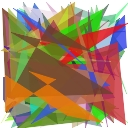
\includegraphics{media/paralell0.jpg}
  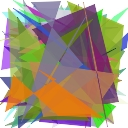
\includegraphics{media/paralell13.jpg}
  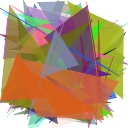
\includegraphics{media/paralell62.jpg}
\end{figure}
\begin{figure}[htp]
  \centering
  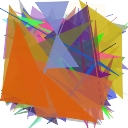
\includegraphics{media/paralell83.jpg}
  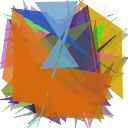
\includegraphics{media/paralell111.jpg}
  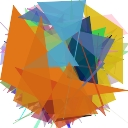
\includegraphics{media/paralell188.jpg}
\end{figure}

\subsection{Corrida paralelizada}
\label{sec:cor-paralelizada}

\begin{itemize}
\item \textbf{Tiempo de CPU:} 116min 20seg.
\item \textbf{Cantidad de imágenes generadas:} 188 imágenes.
\item \textbf{Máximo fitness alcanzado:} 89.850616\%
\end{itemize}

\begin{figure}[htp]
  \centering
  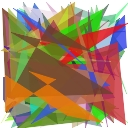
\includegraphics{media/paralell0.jpg}
  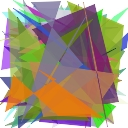
\includegraphics{media/paralell13.jpg}
  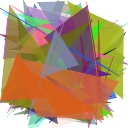
\includegraphics{media/paralell62.jpg}
\end{figure}
\begin{figure}[htp]
  \centering
  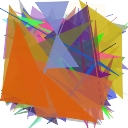
\includegraphics{media/paralell83.jpg}
  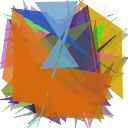
\includegraphics{media/paralell111.jpg}
  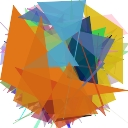
\includegraphics{media/paralell188.jpg}
\end{figure}

\section{Análisis de resultados y conclusiones}
\label{sec:conclusiones}



\bibliographystyle{plain}
\bibliography{evolve_refs}
\end{document}
